% Escribe aquí tu parte. NO toques el main.
% Usa \section{}, \subsection{}, etc.
% Para imágenes usa: \includegraphics[width=\linewidth]{figures/TU_CARPETA/imagen.png}
\chapter{Modelo Documental (Javi)}

El modelo documental es una extensión del modelo clave-valor donde el valor es un documento estructurado (generalmente JSON, BSON o XML) que el sistema de base de datos puede entender, consultar e indexar. Para esta práctica, se ha elegido **MongoDB**, el gestor de base de datos NoSQL orientado a documentos más popular del mercado.

\section{Instalación y Configuración del Entorno}
Dado que el entorno de desarrollo se basa en sistemas Linux, se detalla el proceso de instalación tanto para distribuciones basadas en Arch Linux (sistema del alumno) como para Ubuntu/Debian (sistema de referencia).

\subsection{Instalación en Arch Linux}
En Arch Linux, los paquetes de MongoDB se encuentran gestionados a través del repositorio de usuarios (AUR), ya que la licencia cambió hace unas versiones.

\begin{enumerate}
    \item \textbf{Instalación del servidor:} Se utiliza un ayudante de AUR (como \texttt{yay}) para instalar los binarios:
    \begin{verbatim}
    yay -S mongodb-bin
    \end{verbatim}
    \item \textbf{Instalación de la GUI (opcional):} De igual forma, instalamos la interfaz gráfica oficial:
    \begin{verbatim}
    yay -S mongodb-compass
    \end{verbatim}
    \item \textbf{Inicio del servicio:} Habilitamos y arrancamos el demonio con systemd:
    \begin{verbatim}
    sudo systemctl enable --now mongodb
    \end{verbatim}
\end{enumerate}

\subsection{Instalación en Ubuntu/Debian}
Para sistemas basados en Debian, se puede cargar directamente usando el .deb.

\begin{enumerate}
    \item \textbf{Instalación de herramientas:}
    \begin{verbatim}
      sudo apt-get install gnupg curl
    \end{verbatim}
    \item \textbf{Importar la GPG key de MongoDB:}
    \begin{verbatim}
      curl -fsSL https://www.mongodb.org/static/pgp/server-7.0.asc | \
      sudo gpg -o /usr/share/keyrings/mongodb-server-7.0.gpg \
      --dearmor
    \end{verbatim}
    \item \textbf{Crear el archivo de lista correspondiente:}
    \begin{tabbing}
      echo "deb [ arch=amd64,arm64 \\signed-by=/usr/share/keyrings/mongodb-server-7.0.gpg ] \\https://repo.mongodb.org/apt/ubuntu jammy/mongodb-org/7.0 multiverse"\\ | sudo tee /etc/apt/sources.list.d/mongodb-org-7.0.list
    \end{tabbing}


    \item \textbf{Recargar base de datos y descargar mongodb:}
    \begin{verbatim}
      sudo apt-get update && sudo apt-get install -y mongodb-org
    \end{verbatim}
    \item \textbf{Descargar el .deb de la GUI (opcional):}
    \begin{verbatim}
      wget 
      https://downloads.mongodb.com/compass/mongodb-compass_1.46.10_amd64.deb
    \end{verbatim}
    \item \textbf{Instalar la GUI usando apt:}
    \begin{verbatim}
      sudo apt install ./mongodb-compass_1.46.10_amd64.deb
    \end{verbatim}
\end{enumerate}

\begin{figure}[h]
    \centering
    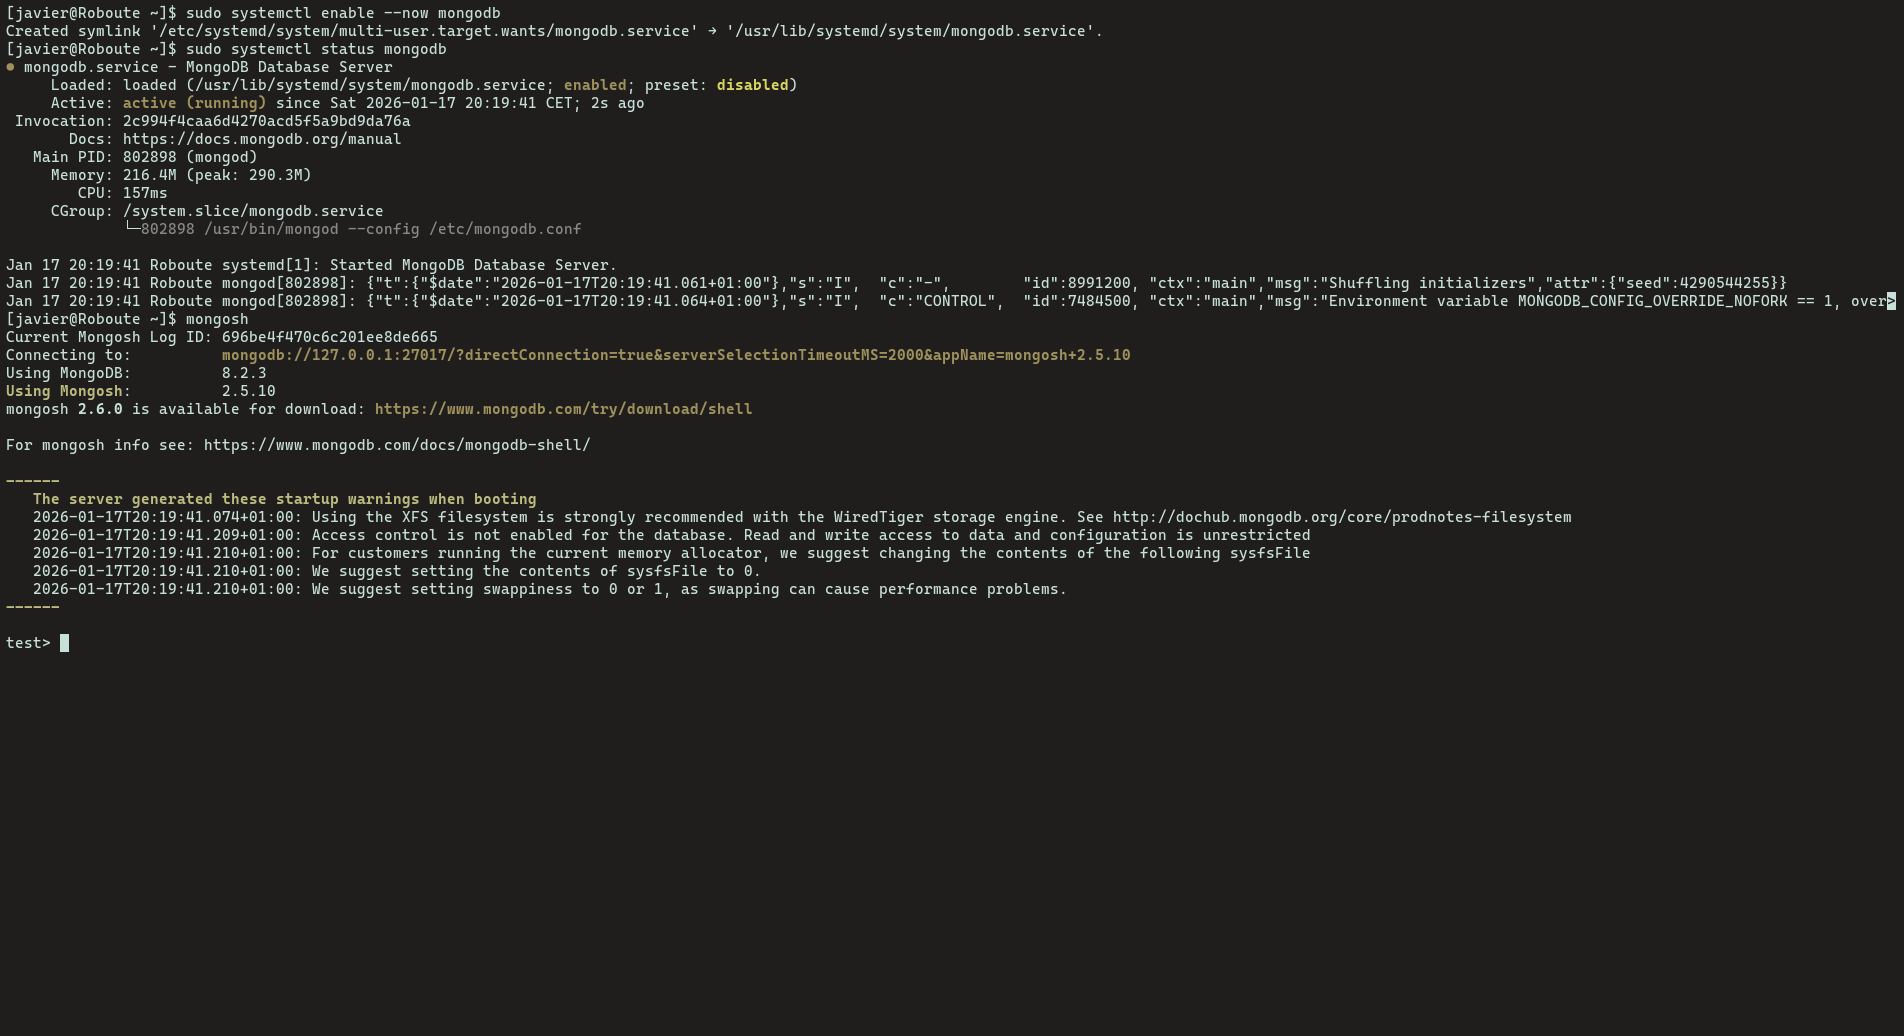
\includegraphics[width=\linewidth]{figures/javier/mongo_install_linux.png} 
    \caption{Shell de MongoDB ejecutándose en entorno Linux.}
    \label{fig:mongo_install}
\end{figure}

\section{Descripción del DDL y DML en MongoDB}
A diferencia de SQL, MongoDB no requiere una definición estricta de esquema (DDL explícito) antes de insertar datos. Las colecciones se crean automáticamente cuando se inserta el primer documento. No obstante, dispone de comandos equivalentes:

\begin{itemize}
    \item \textbf{DDL (Definición):}
    \begin{itemize}
        \item \texttt{use <db>}: Selecciona la base de datos (o la crea si no existe).
        \item \texttt{db.createCollection()}: Crea una colección explícitamente (opcional).
        \item \texttt{db.collection.drop()}: Elimina una colección (equivalente a \texttt{DROP TABLE}).
    \end{itemize}
    \item \textbf{DML (Manipulación):}
    \begin{itemize}
        \item \texttt{db.collection.insertOne()}: Equivalente a \texttt{INSERT}. Guarda documentos en formato BSON.
        \item \texttt{db.collection.find()}: Equivalente a \texttt{SELECT}. Permite filtrar por campos, incluso dentro de arrays o subdocumentos.
        \item \texttt{db.collection.updateOne()}: Equivalente a \texttt{UPDATE}. Utiliza operadores atómicos como \texttt{\$set} o \texttt{\$inc}.
        \item \texttt{db.collection.deleteOne()}: Equivalente a \texttt{DELETE}.
    \end{itemize}
\end{itemize}

\section{Implementación de Estructuras y Pruebas}
Para simular el subsistema de \textbf{Publicaciones} de EKIS en un modelo documental, aprovecharemos la capacidad de anidamiento. En lugar de tener tablas separadas para \texttt{PUBLICACION}, \texttt{HASHTAGS} y \texttt{COMENTARIOS} (como en el relacional), podemos tener una única colección \texttt{posts} donde cada documento contiene toda la información.

\subsection{Inserción de Datos (Creación)}
Creamos una publicación que incluye arrays para los hashtags y un subdocumento para la ubicación, demostrando la flexibilidad del esquema.
Las inserciones se pueden hacer desde la terminal o usando un .js en el que se definen las órdenes a ejecutar. De ahí se pasa a mongosh por entrada estándar.

\begin{lstlisting}[language=bash, caption={Inserción de una publicación con estructura compleja}]
use ekis_doc

db.publicaciones.insertOne({
  titulo: "Atardecer en la Alhambra",
  descripcion: "Disfrutando de las vistas con amigos.",
  usuario: "javier_ns",
  fecha: new Date(),
  likes: 0,
  tags: ["granada", "alhambra", "relax"],
  ubicacion: {
    ciudad: "Granada",
    lat: 37.176,
    lon: -3.588
  },
  comentarios: [] 
})
\end{lstlisting}

\begin{figure}[h]
    \centering
    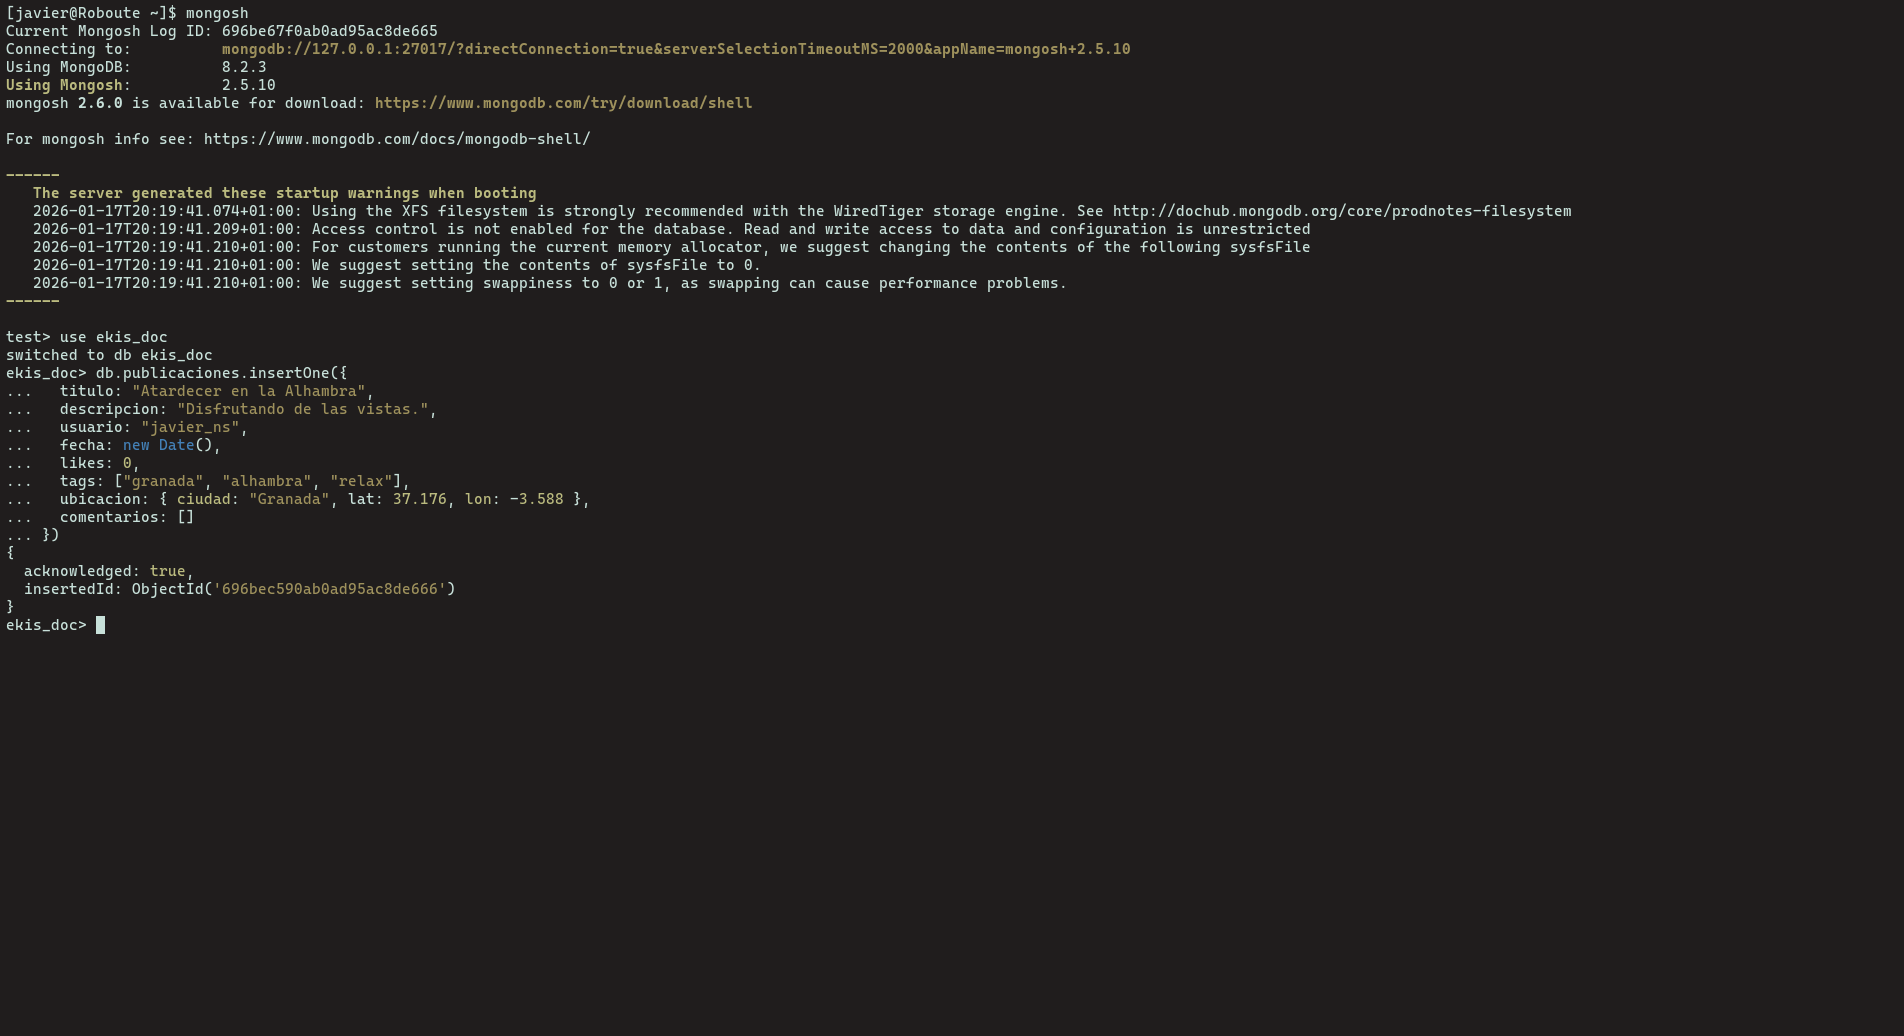
\includegraphics[width=\linewidth]{figures/javier/mongo_insert.png}
    \caption{Nueva publicación insertada en la colección \texttt{publicaciones}.}
    \label{fig:mongo_insert}
\end{figure}
\newpage
\subsection{Consultas (Lectura)}
Realizamos una consulta para buscar todas las publicaciones que contengan el tag "granada". Esto equivale a un \texttt{SELECT} con \texttt{JOIN} en SQL, pero aquí es una búsqueda directa sobre el array.

\begin{lstlisting}[language=bash, caption={Consulta por etiqueta (tag)}]
db.publicaciones.find({ tags: "granada" })
\end{lstlisting}

\begin{figure}[h]
    \centering
    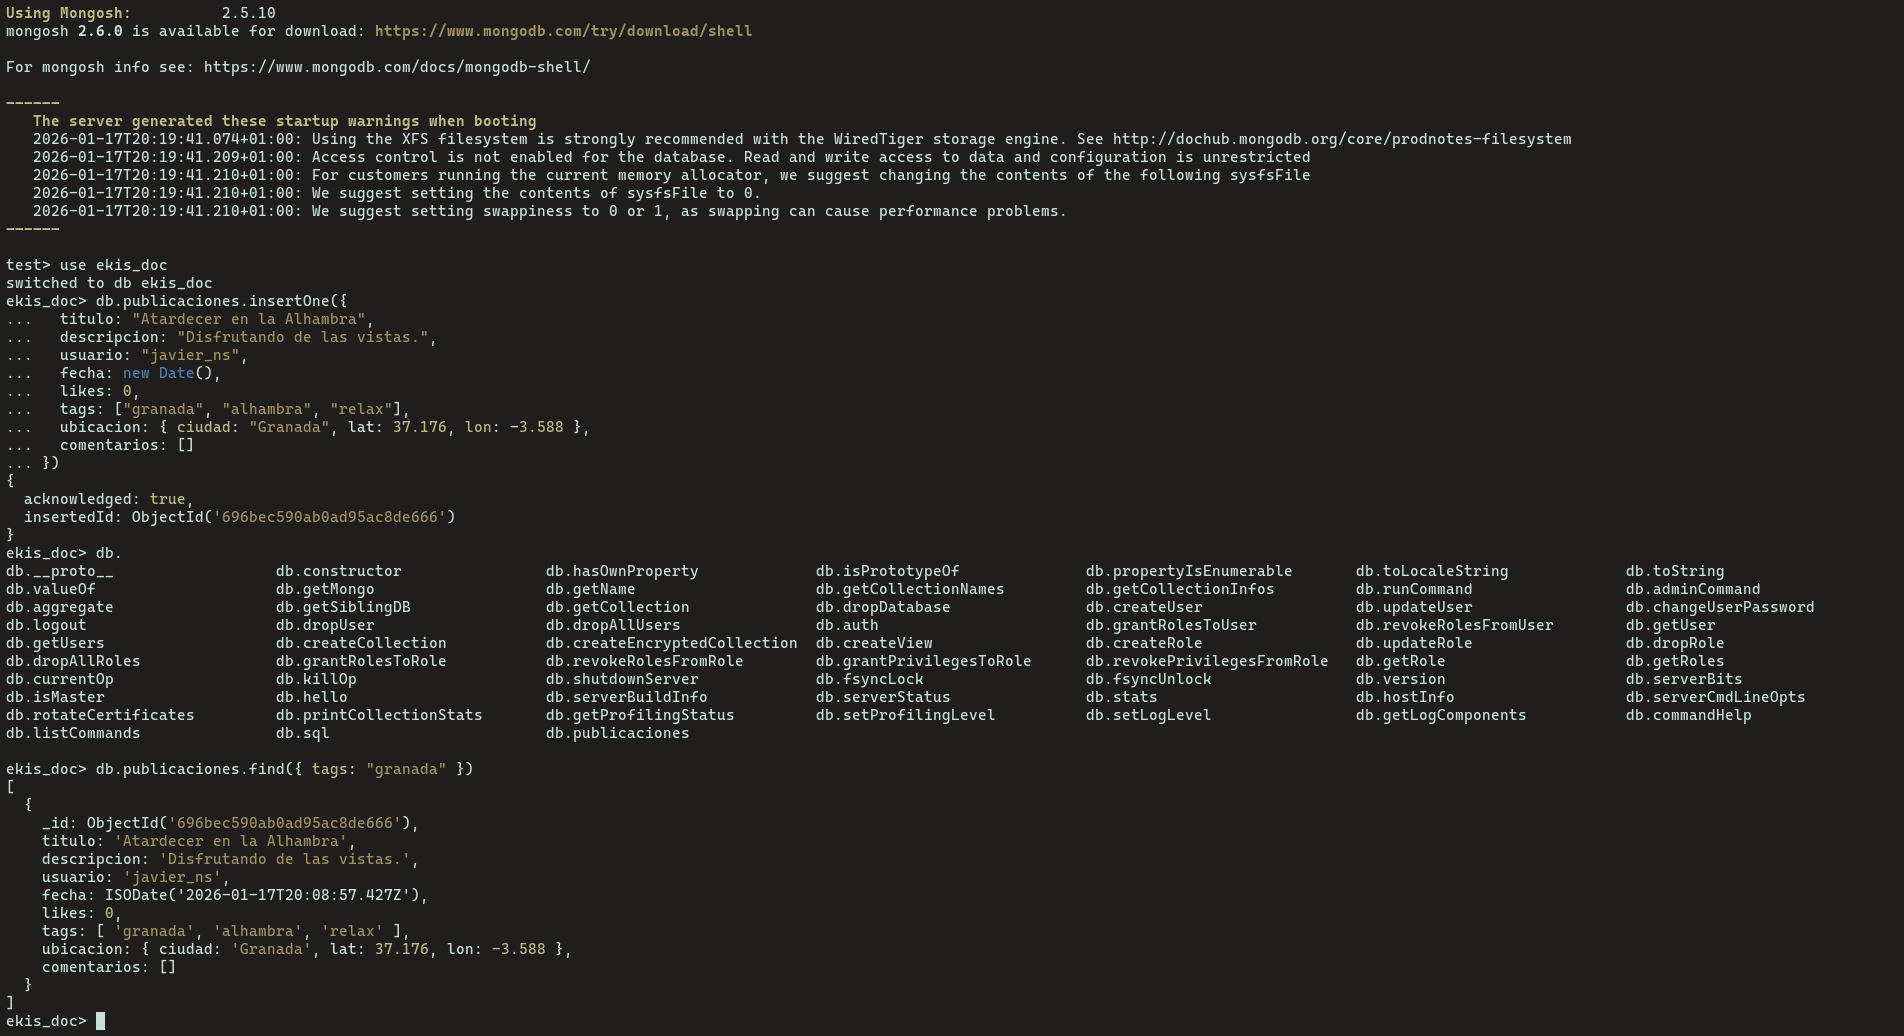
\includegraphics[width=\linewidth]{figures/javier/mongo_find.png}
    \caption{Resultado de la consulta filtrando por tags.}
    \label{fig:mongo_find}
\end{figure}
\newpage
\subsection{Modificación y Actualización}
Simulamos la acción de "Dar Like". En MongoDB podemos usar el operador \texttt{\$inc} para incrementar el contador atómicamente y \texttt{\$push} para añadir un comentario simultáneamente.

%TODO: Poner los acentos, ahora mismo se han quitado para que no den errores
\begin{lstlisting}[language=bash, caption={Actualizacion atomica: Like y Comentario}]
db.publicaciones.updateOne(
  { usuario: "javier_ns" },
  { 
    $inc: { likes: 1 },
    $push: { comentarios: { 
        usuario: "ismael_sm", 
        texto: "!Foton!",
        fecha: new Date() 
    }}
  }
)
\end{lstlisting}

\begin{figure}[h]
    \centering
    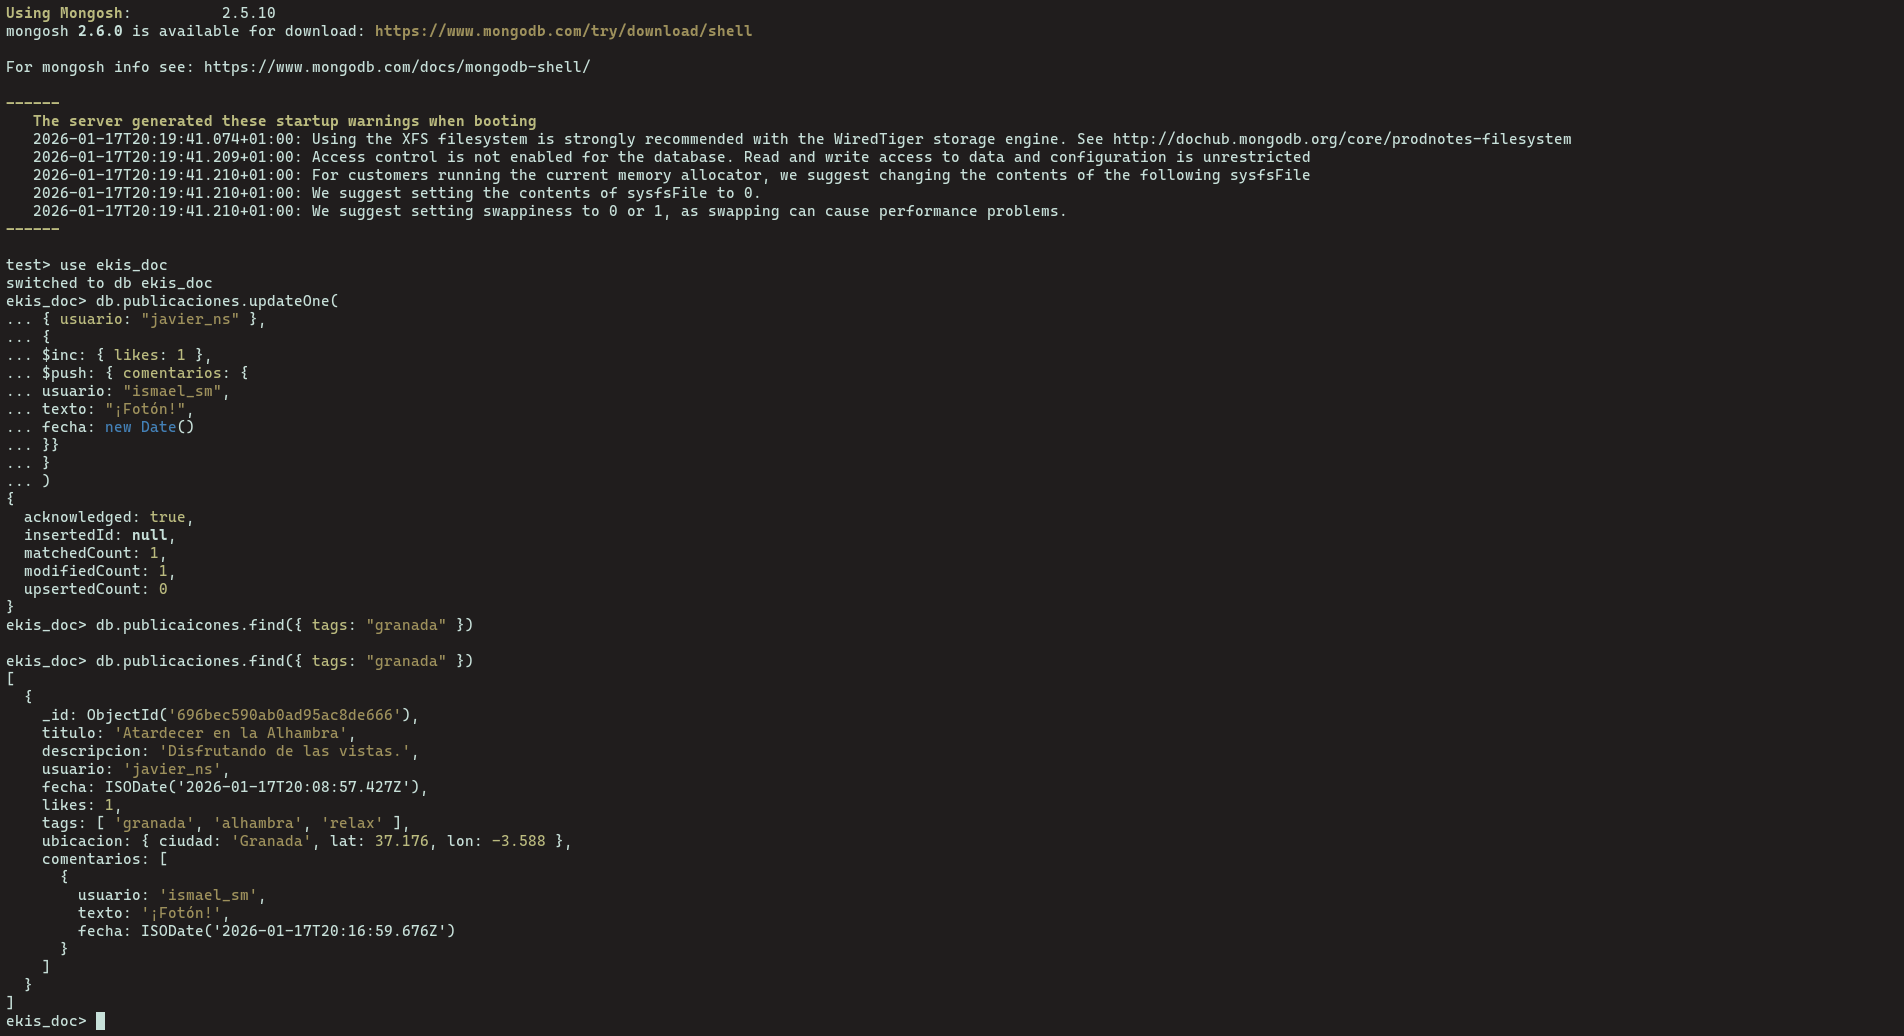
\includegraphics[width=\linewidth]{figures/javier/mongo_edit.png}
    \caption{Resultado edición de publicación.}
    \label{fig:mongo_edit}
\end{figure}
\newpage
\subsection{Borrado}
Finalmente, eliminamos la publicación creada.

\begin{lstlisting}[language=bash, caption={Eliminación del documento}]
db.publicaciones.deleteOne({ usuario: "javier_ns" })
\end{lstlisting}

\begin{figure}[h]
    \centering
    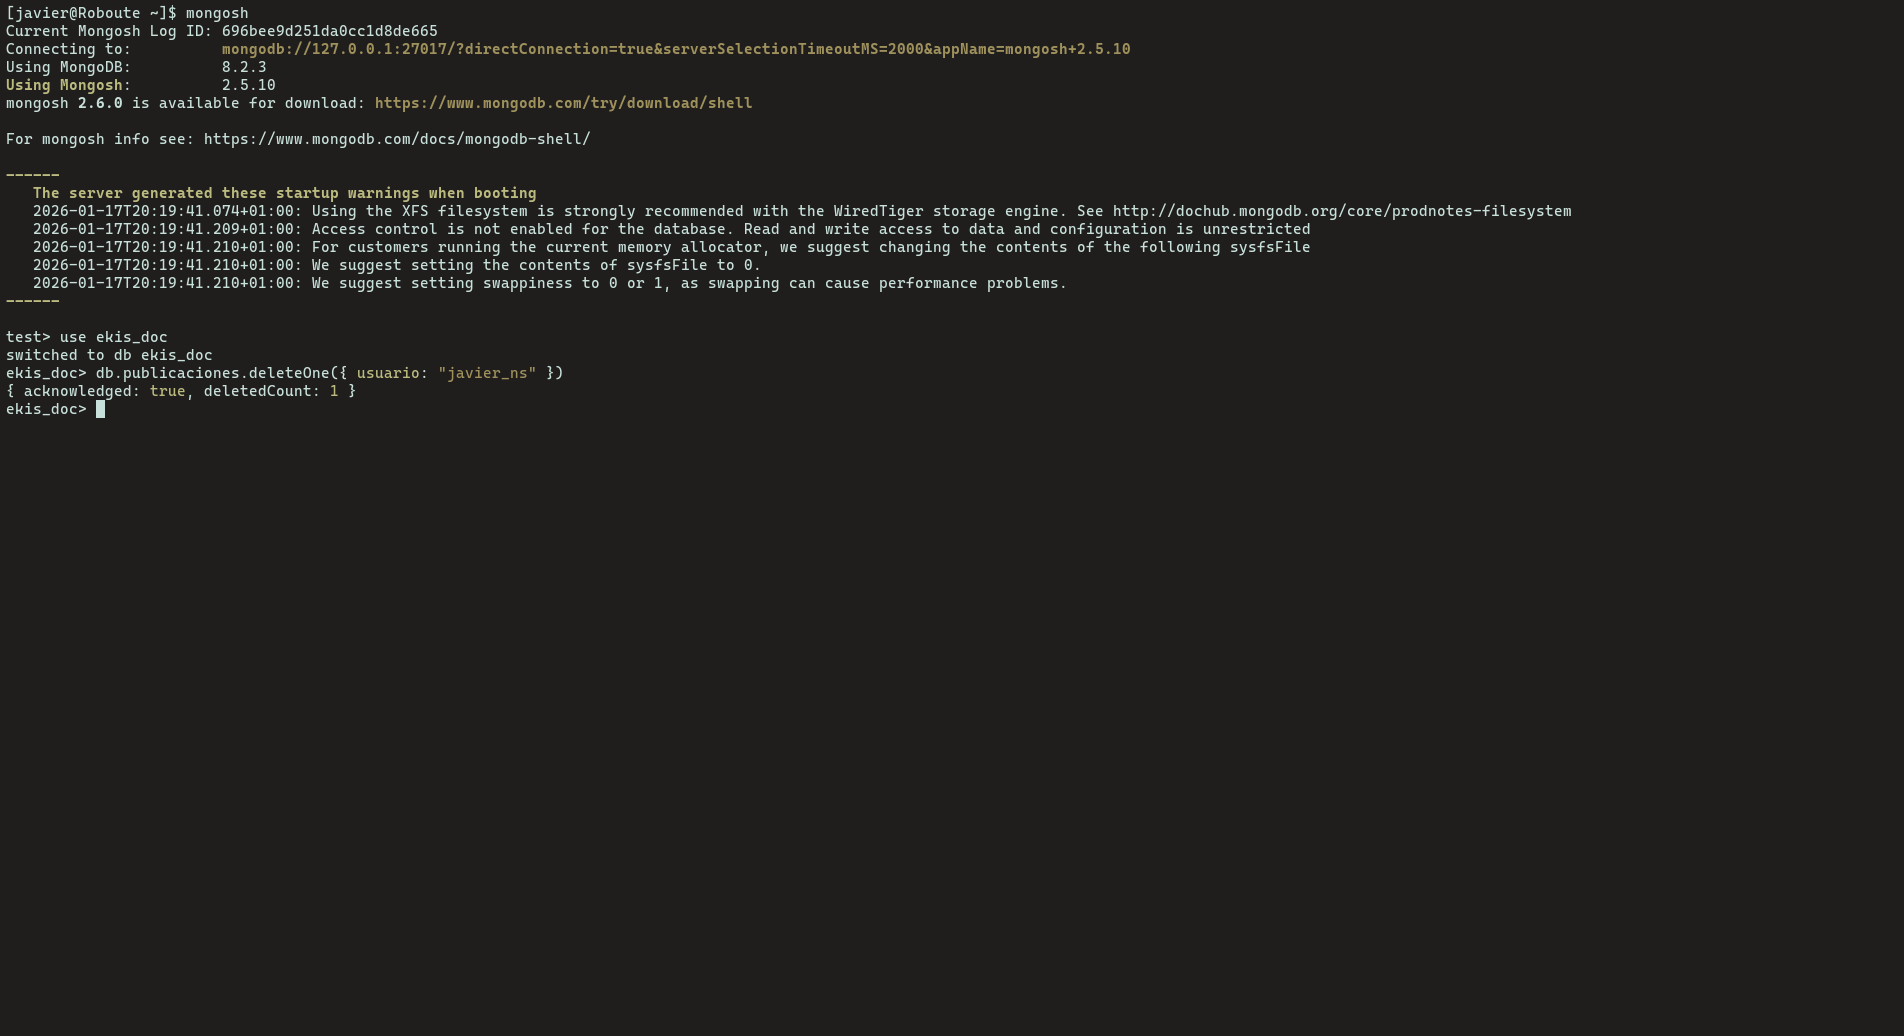
\includegraphics[width=\linewidth]{figures/javier/mongo_delete.png}
    \caption{Resultado de eliminación de publicación.}
    \label{fig:mongo_delete}
\end{figure}
\newpage
\section{Adecuación al Sistema EKIS}
El uso de un modelo documental con MongoDB presenta ventajas significativas para el subsistema de Publicaciones de una red social como EKIS:

\begin{itemize}
    \item \textbf{Flexibilidad de Esquema:} Las publicaciones pueden evolucionar. Algunos posts pueden tener encuestas, otros solo texto, y otros imágenes. SQL obliga a tener columnas nulas o muchas tablas; MongoDB permite que cada documento tenga campos distintos.
    \item \textbf{Rendimiento en Lectura (Feed):} Al guardar los comentarios y tags \textit{embebidos} dentro de la publicación, podemos recuperar toda la información necesaria para pintar el "Muro" con una sola lectura de disco, evitando los costosos \texttt{JOINS} del modelo relacional.
    \item \textbf{Escalabilidad:} Las redes sociales generan un volumen masivo de datos. MongoDB facilita el escalado horizontal (\textit{sharding}), distribuyendo las publicaciones en varios servidores de forma transparente.
\end{itemize}

Sin embargo, para datos altamente transaccionales y estructurados como la facturación de publicidad o la gestión estricta de usuarios, el modelo relacional sigue siendo superior por sus garantías ACID estrictas.
